Gapminder\footnote{See \href{https://www.gapminder.org/}{Gapminder online}} is very well known in the information visualisation community and the content of the data it uses is entirely explored. It shows wealth and health of countries over time and has more than 500 datasets as a basis. The default visualisation of gapminder is an extended scatter plot where the x-axis shows income per person, the y-axis life expectancy in years, the bubble itself represents the total population of each country by size and the color indicates the region of the country. Furthermore, the scatter plot is expanded with a timeline. The interactive demo of Gapminder also allows users to inspect different indicators of wealth and health.

\begin{figure}[!htb]
\centering
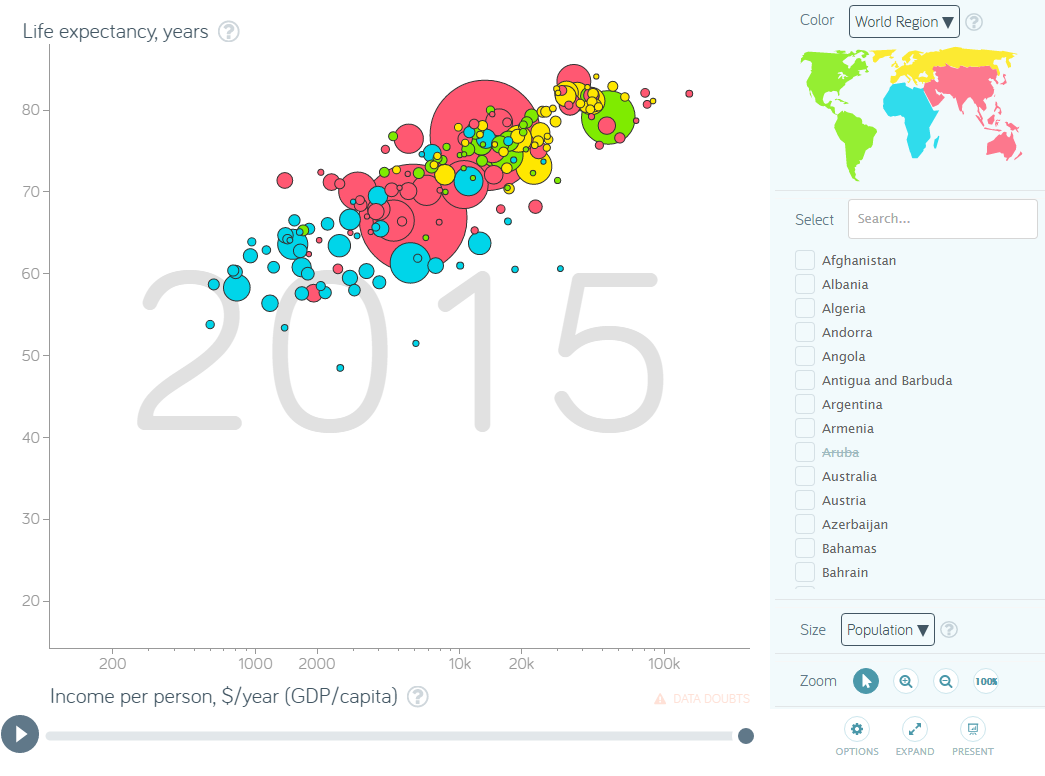
\includegraphics[height=5cm]{images/methods/related/gapminder.png}
\caption[
    Gapminder
]{Gapminder}
\label{fig:gapminder}
\end{figure}

Gapminder is not visualisation tool, but demonstrates a very popular example of animation in visualisations as a practical example. Figure \ref{fig:gapminder} on page \pageref{fig:gapminder} shows the application displaying the data corresponding to the year 1904. Users have some control over the visualisation shown:
\begin{itemize}
\item changing the attributes mapped,
\item controlling the animation by playing and pausing it directly,
\item selecting the countries which are of interest and
\item setting the symbol size.
\end{itemize}

The application made it possible to discover that people live longer in countries with a higher \ac{GDP} per capita. Countries with a low income have really short life expectancy. Furthermore, it is also discovered, that living in middle-income countries, the lifespan is huge, depending on how the income in the country is distributed and used.
